\chapter{Appendix A}
\lhead{\emph{Appendix A}}

\section{Introduction}

Appendix Introduction

The appendix of this thesis provides a more detailed look at the technical aspects of the research presented in the main body. This includes supporting charts, visualizations, and code snippets that explain the specific pre-processing steps, Optical Character Recognition (OCR) techniques, and font selection choices that were made.

The materials in this appendix are not essential for understanding the main findings of the thesis, but they are important for readers who want a deeper understanding of the methods and processes used. This is especially true for the novel pre-processing steps and the role of image quality and contrast in OCR.

By navigating through this appendix, enthusiasts and specialists alike will gain a deeper understanding of the intricacies that have contributed to the efficacy of the OCR approach undertaken in this Thesis.

\newpage

\section{Analysis Tesseract Separate Folders}

\subsection{Image Folder A Best Image Size Analysis}

\begin{figure}[ht]
    \centering
    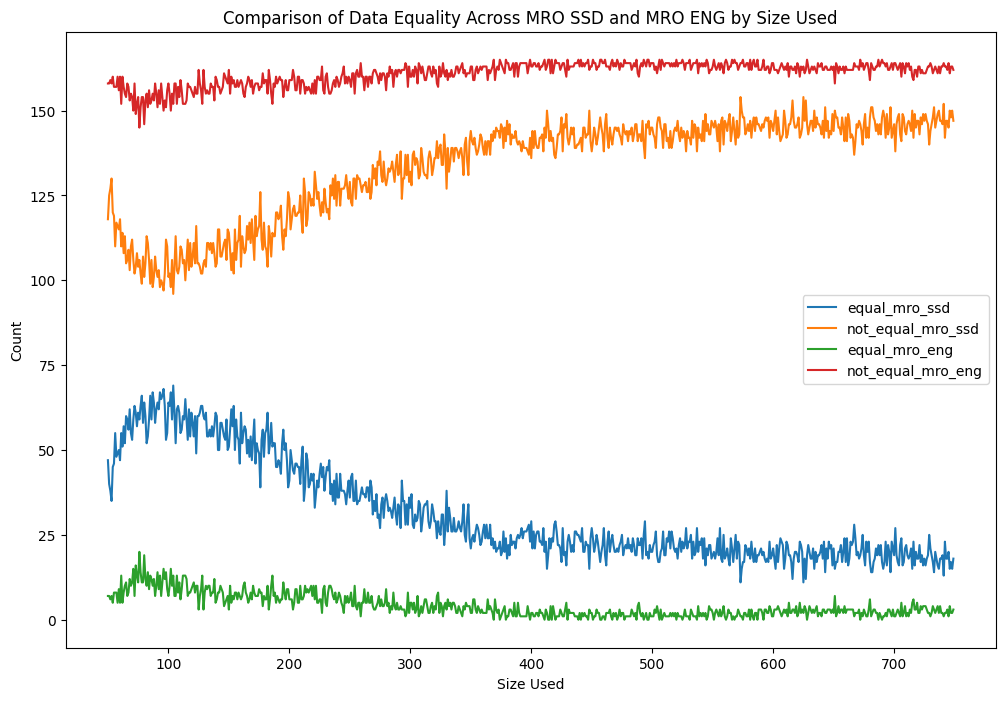
\includegraphics[width=0.9\textwidth]{Figures/Results/sipa_02/count_analysis.png}
    \caption[Count Analysis]{Image Folder A Count Analysis}
    \label{fig:Image Folder A Best Image Size Analysis}
\end{figure}

The chart presented primarily emphasizes the blue line, which signifies the count of Masked Red OTSU. This line is of particular importance. At size 104, we observe the peak read count.

This establishes the dimensions to which the images will be resized for each of the subsequent directories.

\newpage




\newpage

\subsection{Image Folder A Contrast Analysis on MRO SSD}

\begin{figure}[ht]
    \centering
    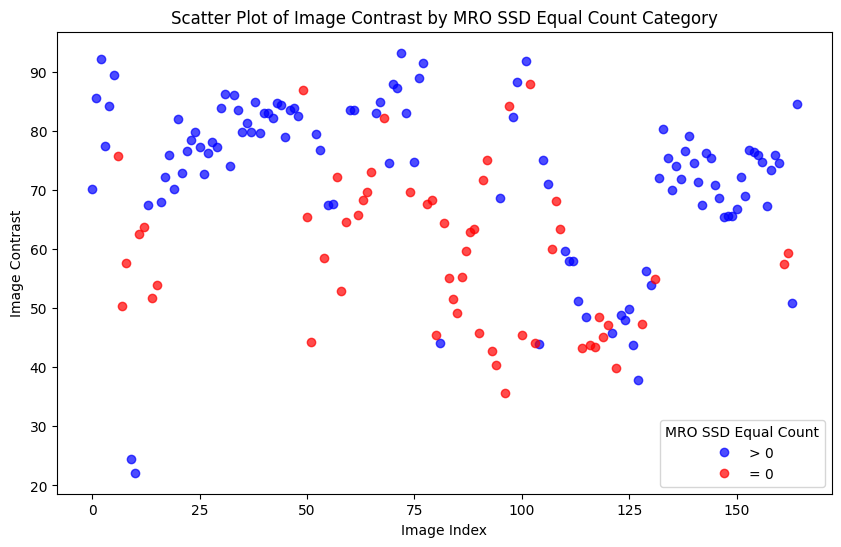
\includegraphics[width=0.9\textwidth]{Figures/Results/sipa_02/contrast.png}
    \caption[Image Folder A Contrast Analysis on MRO SSD]{Image Folder A Contrast Analysis on MRO SSD}
    \label{fig:Image Folder A Contrast Analysis on MRO SSD}
\end{figure}

The scatter plot of image contrast shows that there is a wide range of contrast levels for both categories of images (MRO SSD EQUAL COUNT greater than 0 and equal to 0). This means that the contrast of images in both categories is highly variable. Additionally, there is significant overlap in the contrast values of both categories, suggesting that the contrast of an image may not be a strong indicator of whether the MRO SSD EQUAL COUNT is greater than 0 or not.

There are a few outliers in the MRO SSD EQUAL COUNT greater than 0 category with particularly high contrast levels. However, these outliers do not significantly change the overall pattern of the scatter plot.

In summary, the scatter plot of image contrast does not provide any clear evidence that the contrast of an image is a good predictor of the MRO SSD EQUAL COUNT value.

\newpage

\subsection{Image Folder A Brightness Analysis on MRO SSD}


\begin{figure}[ht]
    \centering
    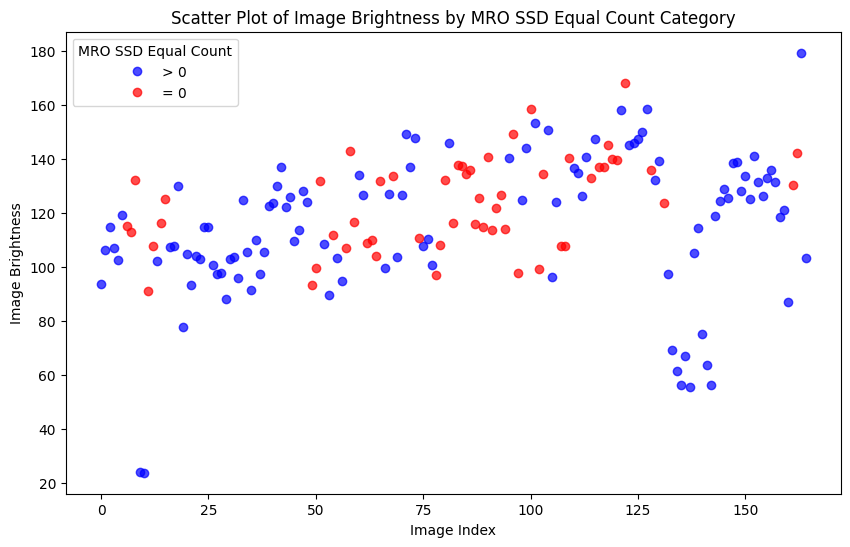
\includegraphics[width=0.9\textwidth]{Figures/Results/sipa_02/brightness.png}
    \caption[Image Folder A Brightness Analysis on MRO SSD]{Image Folder A Brightness Analysis on MRO SSD}
    \label{fig:Image Folder A Brightness Analysis on MRO SSD}
\end{figure}



The scatter plot of image brightness shows that both categories of images (MRO SSD EQUAL COUNT greater than 0 and equal to 0) have a wide range of brightness values. This means that the brightness of images in both categories is highly variable. Additionally, there is no clear pattern or correlation between the MRO SSD EQUAL COUNT category and the brightness of the images. This suggests that the brightness of an image may not be a good predictor of whether the MRO SSD EQUAL COUNT is greater than 0 or not.

There are a few outliers in the MRO SSD EQUAL COUNT greater than 0 category with particularly high brightness levels. However, these outliers do not significantly change the overall pattern of the scatter plot.

In summary, the scatter plot of image brightness does not provide any clear evidence that the brightness of an image is a good predictor of the MRO SSD EQUAL COUNT value.

\newpage

\subsection{Image Folder A Standard Deviation Analysis on MRO SSD}


\begin{figure}[ht]
    \centering
    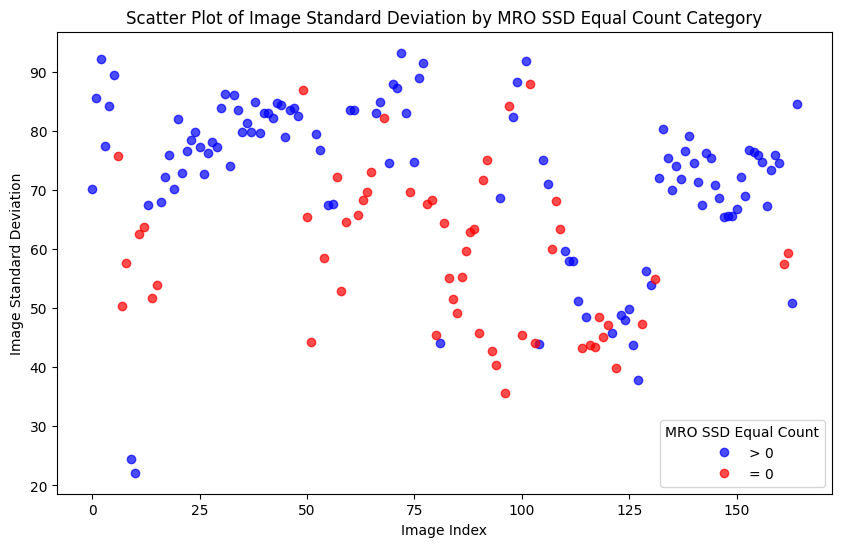
\includegraphics[width=0.9\textwidth]{Figures/Results/sipa_02/sd.png}
    \caption[Image Folder A Standard Deviation Analysis on MRO SSD]{Image Folder A Standard Deviation Analysis on MRO SSD}
    \label{fig:Image Folder A Standard Deviation Analysis on MRO SSD}
\end{figure}

The scatter plot of image standard deviation shows that there is a wide range of standard deviations for both categories of images (MRO SSD EQUAL COUNT greater than 0 and equal to 0). This means that the spread of pixel values within the images is highly variable. Additionally, there is significant overlap in the standard deviation values of both categories, suggesting that the standard deviation of pixel values within an image may not be a strong indicator of whether the MRO SSD EQUAL COUNT is greater than 0 or not.


\newpage

\subsection{Image Folder A Homogeneity Analysis on MRO SSD}


\begin{figure}[ht]
    \centering
    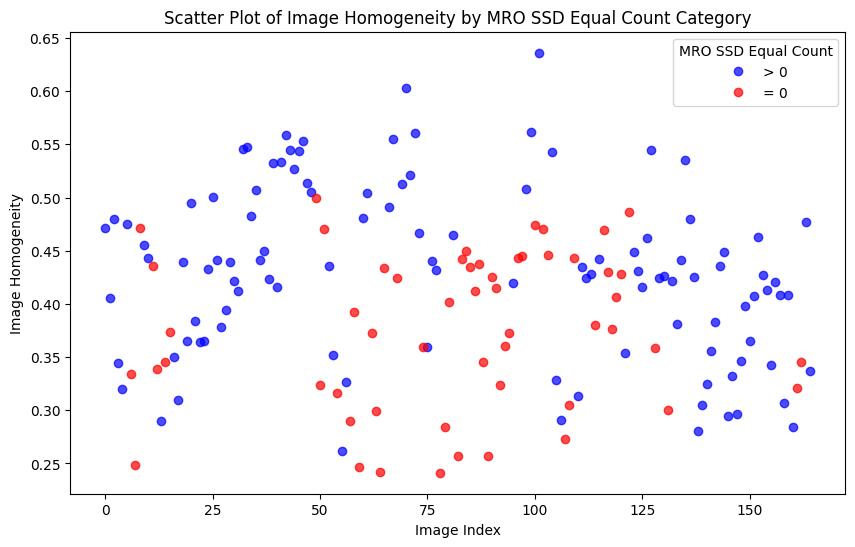
\includegraphics[width=0.9\textwidth]{Figures/Results/sipa_02/homogeneity.png}
    \caption[Image Folder A Homogeneity Analysis on MRO SSD]{Image Folder A Homogeneity Analysis on MRO SSD}
    \label{fig:Image Folder A Homogeneity Analysis on MRO SSD}
\end{figure}


The scatter plot of image Homogeneity shows that there is a wide range of homogeneity levels for both categories of images (MRO SSD EQUAL COUNT greater than 0 and equal to 0). This signifies that the homogeneity of images in both categories is highly variable. Additionally, there is significant overlap in the homogeneity values of both categories, suggesting that the homogeneity of an image may not be a strong indicator of whether the MRO SSD EQUAL COUNT is greater than 0 or not.



In summary, the scatter plot of image homogeneity does not provide any clear evidence that the homogeneity of an image is a good predictor of the MRO SSD EQUAL COUNT value.

\newpage

\subsection{Image Folder A Sharpness Analysis on MRO SSD}


\begin{figure}[ht]
    \centering
    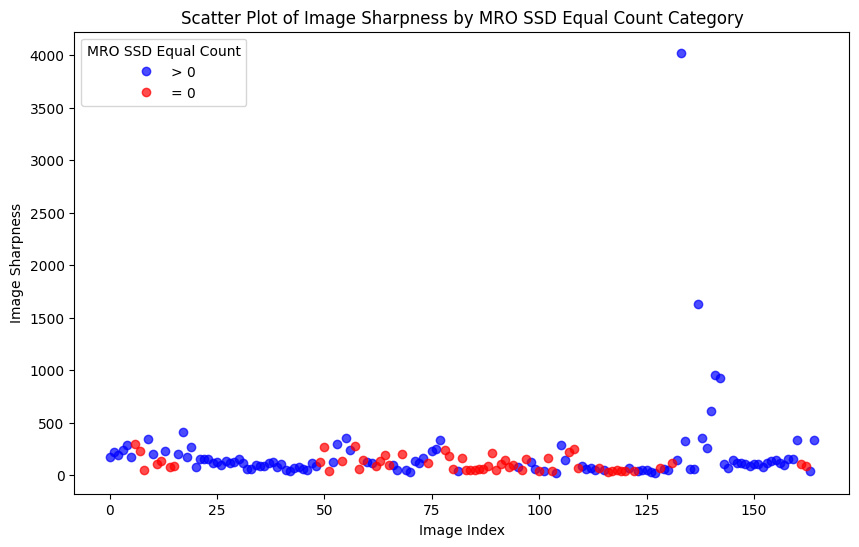
\includegraphics[width=0.9\textwidth]{Figures/Results/sipa_02/sharpness.png}
    \caption[Image Folder A Sharpness Analysis on MRO SSD]{Image Folder A Sharpness Analysis on MRO SSD}
    \label{fig:Image Folder A Sharpness Analysis on MRO SSD}
\end{figure}



The scatter plot of image Sharpness shows that there is a narrow range of sharpness levels for both categories of images (MRO SSD EQUAL COUNT greater than 0 and equal to 0). This signifies that the sharpness of images in both categories is reasonably uniform. Additionally, there is significant overlap in the sharpness values of both categories, suggesting that the sharpness of an image may not be a strong indicator of whether the MRO SSD EQUAL COUNT is greater than 0 or not.

In summary, the scatter plot of image sharpness does not provide any clear evidence that the sharpness of an image is a good predictor of the MRO SSD EQUAL COUNT value.

\newpage


\subsection{Image Folder A Dissimilarity Analysis on MRO SSD}


\begin{figure}[ht]
    \centering
    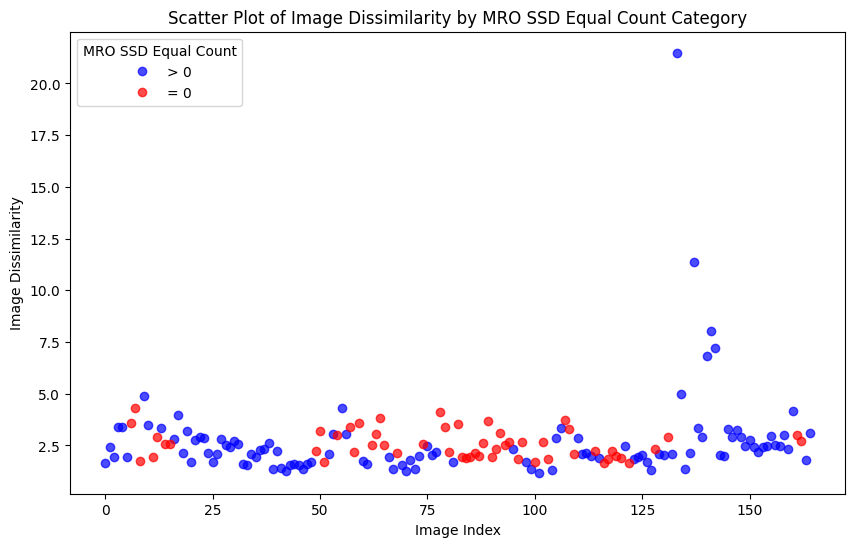
\includegraphics[width=0.9\textwidth]{Figures/Results/sipa_02/dissimilarity.png}
    \caption[Image Folder A Dissimilarity Analysis on MRO SSD]{Image Folder A Dissimilarity Analysis on MRO SSD}
    \label{fig:Image Folder A Dissimilarity Analysis on MRO SSD}
\end{figure}



The scatter plot of image Dissimilarity shows that there is a narrow range of dissimilarity levels for both categories of images (MRO SSD EQUAL COUNT greater than 0 and equal to 0). This signifies that the dissimilarity of images in both categories is reasonably uniform. Additionally, there is significant overlap in the dissimilarity values of both categories, suggesting that the dissimilarity of an image may not be a strong indicator of whether the MRO SSD EQUAL COUNT is greater than 0 or not.

In summary, the scatter plot of image dissimilarity does not provide any clear evidence that the dissimilarity of an image is a good predictor of the MRO SSD EQUAL COUNT value.


\newpage

\subsection{Image Folder A Area Analysis on MRO SSD}


\begin{figure}[ht]
    \centering
    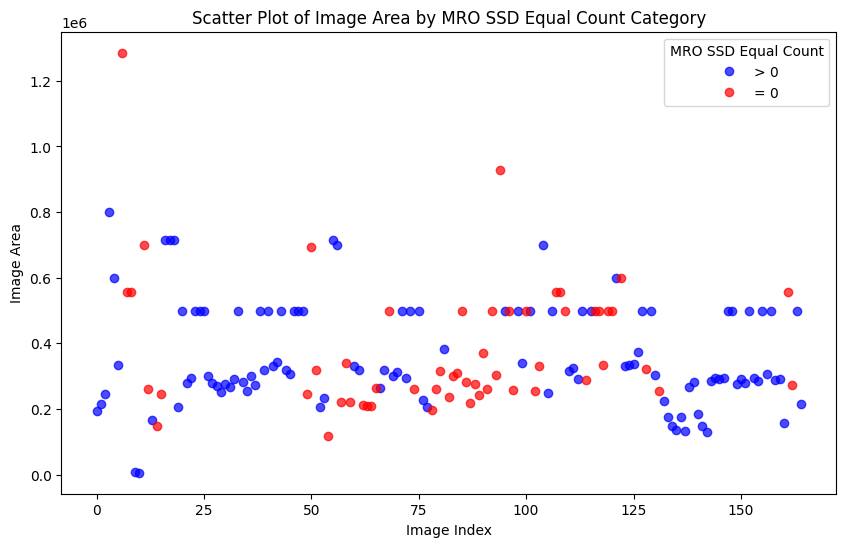
\includegraphics[width=0.9\textwidth]{Figures/Results/sipa_02/area.png}
    \caption[Image Folder A Area Analysis on MRO SSD]{Image Folder A Area Analysis on MRO SSD}
    \label{fig:Image Folder A Area Analysis on MRO SSD}
\end{figure}


The distribution of image area values for both categories (> 0 and = 0) is wide. However, the distribution appears to be slightly different for the two categories, with a higher density of points at lower image area values for the = 0 category.

There is a significant density of points near the lower end of the image area values for both categories. The = 0 category seems to have a higher density of points at lower image area values.

There is considerable overlap between the two categories, especially at lower image area values. This suggests that while there may be a trend, the MRO SSD EQUAL COUNT value is not a definitive predictor of the image area value.

There appear to be some outliers in the >0 category with high image area values. This suggests that there may be some instances where MRO SSD EQUAL COUNT is greater than 0 and the image area is significantly larger than the typical values.

In summary, this scatter plot suggests that there might be a slight tendency for instances with MRO SSD EQUAL COUNT of 0 to have smaller image areas. However, the relationship is not clear-cut, as there is significant overlap between the two categories.



\newpage

\subsection{Image Folder A Correlation Analysis on MRO SSD}


\begin{figure}[ht]
    \centering
    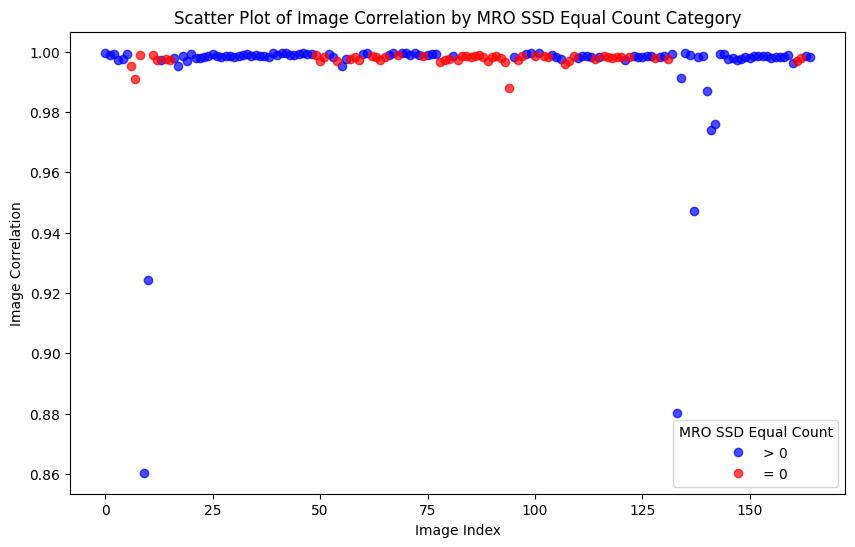
\includegraphics[width=0.9\textwidth]{Figures/Results/sipa_02/correlation.png}
    \caption[Image Folder A Correlation Analysis on MRO SSD]{Image Folder A Correlation Analysis on MRO SSD}
    \label{fig:Image Folder A Correlation Analysis on MRO SSD}
\end{figure}

The distribution of image correlation values for both categories (> 0 and = 0) is varied, similar to the previous plot.

The density of points for both categories appears to be quite uniform across the range of image correlation values. There is perhaps a slightly higher density at lower correlation values for the = 0 category.

There is significant overlap between the two categories across the entire range of image correlation values. This suggests that the MRO SSD EQUAL COUNT value does not strongly distinguish between different levels of image correlation.

There do not seem to be any clear outliers in this plot, unlike the previous plot for Image Energy.

In summary, while there might be a slight tendency for instances with MRO SSD EQUAL COUNT of 0 to have lower image correlation, the relationship is not clear-cut. There is substantial overlap between the two categories, indicating that MRO SSD EQUAL COUNT may not be a strong predictor for image correlation.

\newpage

\subsection{Image Folder A Energy Analysis on MRO SSD}


\begin{figure}[ht]
    \centering
    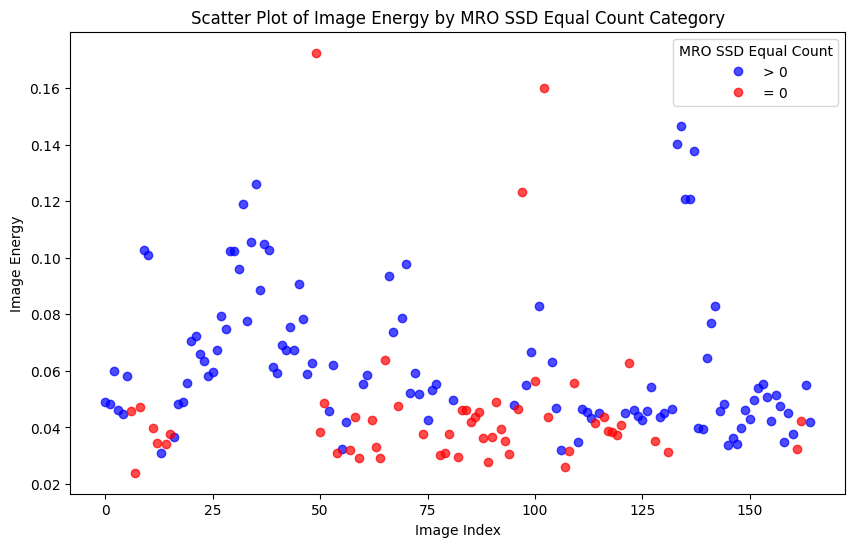
\includegraphics[width=0.9\textwidth]{Figures/Results/sipa_02/energy.png}
    \caption[Image Folder A Energy Analysis on MRO SSD]{Image Folder A Energy Analysis on MRO SSD}
    \label{fig:Image Folder A Energy Analysis on MRO SSD}
\end{figure}




The distribution of Image Energy values for both categories (> 0 and = 0) is quite scattered. This suggests that the distribution of energy values is varied for both cases.

There appears to be a higher density of red points (= 0 category) towards the lower Image Energy values. This suggests that when MRO SSD EQUAL COUNT is zero, the image energy tends to be lower.

There are some apparent outliers in the blue category (gt 0), with significantly higher Image Energy values. This suggests that there might be a few instances with MRO SSD EQUAL COUNT greater than 0 that have unusually high image energy.

There is considerable overlap between the two categories. This indicates that while there might be a general trend (as indicated in points 2 and 3), the MRO SSD EQUAL COUNT value is not a definitive predictor of the Image Energy value.

\newpage

\subsection{Mask Red Function}
% \begin{singlespacing}
\begin{lstlisting}[language=Python, caption=Mask Red Function]

    def mask_red(img):
        """
        Returns an image with only the red pixels from the input image.

        Parameters:
        img (numpy.ndarray): Input image in BGR format.

        Returns:
        numpy.ndarray: Output image with only the red pixels from the input image.

        """
        img_hsv = cv2.cvtColor(img, cv2.COLOR_BGR2HSV)

        # define lower and upper red ranges in HSV
        lower_red1 = np.array([0, 50, 50])
        upper_red1 = np.array([10, 255, 255])
        lower_red2 = np.array([170, 50, 50])
        upper_red2 = np.array([180, 255, 255])

        # create masks with the specified red ranges
        mask1 = cv2.inRange(img_hsv, lower_red1, upper_red1)
        mask2 = cv2.inRange(img_hsv, lower_red2, upper_red2)

        # join the masks
        mask = mask1 + mask2

        # set the output image to zero everywhere except the red mask
        output_img = img.copy()
        output_img[np.where(mask == 0)] = 0

        return output_img


\end{lstlisting}


% \end{singlespacing}

\newpage

\subsection{Mask Green Function}


% \begin{singlespacing}
\begin{lstlisting}[language=Python, caption=Mask Green Function]
    def mask_green(img):
    """
    Returns an image with only the green pixels from the input image.
    
    Parameters:
    img (numpy.ndarray): Input image in BGR format.
    
    Returns:
    numpy.ndarray: Output image with only the green pixels from the input image.
    
    """
    img_hsv = cv2.cvtColor(img, cv2.COLOR_BGR2HSV)
    
    # define range of green color in HSV
    lower_green = np.array([40, 50, 50])
    upper_green = np.array([80, 255, 255])
    
    # create a mask with the specified green range
    mask = cv2.inRange(img_hsv, lower_green, upper_green)
    
    # apply the mask to the image to get the output image
    output_img = cv2.bitwise_and(img, img, mask=mask)
    
    return output_img
    
    
\end{lstlisting}
% \end{singlespacing}




